%% MLP Coursework 4 - Final Report
%% Based on MLP template (ICML 2017 style)

\documentclass{article}
\input{preamble}

\usepackage{enumitem}
\usepackage{caption}
\usepackage{placeins}
\usepackage{float}

\def\groupNumber{G057}
\def\studentNumber{s2286795}

\mlptitlerunning{MLP Coursework 4 -- Final Report (\studentNumber)}

\begin{document}

\twocolumn[
\mlptitle{Comparing Multimodal Fusion Strategies for Fine-Grained\\Grocery Product Identification}
\centerline{\studentNumber}
\vskip 7mm
]
\makeatletter
\chead{\bf\@mlptitlerunning}
\makeatother

% ============================================================================
\begin{abstract}
% ============================================================================
Fine-grained grocery product identification is a persistent accessibility challenge for blind and visually impaired (BVI) users, where visually similar products---such as full-fat and semi-skimmed milk from the same brand---differ only in small textual details on their packaging. In this work, we present a comparative evaluation of four multimodal fusion architectures that combine visual features from a pretrained CNN with OCR-extracted text to perform fine-grained product classification. Specifically, we evaluate concatenation fusion, gated fusion, cross-attention fusion, and a lightweight fuzzy score fusion approach, benchmarking all four against an image-only baseline on the GroceryStoreDataset (81 classes, 5,421 images). To address the challenges of training on a small dataset, we employ aggressive data augmentation, staged encoder pretraining, and systematic text encoder layer freezing as regularisation strategies. Our results show that score fusion achieves 75.61\% top-1 accuracy, outperforming the image-only baseline by 5.5 percentage points and the best neural fusion method (cross-attention, 73.54\%) by 2.1 points. A modality contribution analysis confirms that both modalities contribute to all fusion methods, with cross-attention showing the largest text contribution (+6.26 points) and gated fusion the smallest (+2.34 points), reflecting the gate's learned preference for image features when text is unreliable.
\end{abstract}

% ============================================================================
\section{Introduction}
\label{sec:intro}
% ============================================================================

Grocery product identification is a key accessibility challenge for blind and visually impaired (BVI) users: 41\% of visual questions submitted by blind users involve food items \citep{brady2013visual}, and distinguishing visually similar products---such as different milk fat percentages from the same brand---remains difficult even for state-of-the-art vision-language models \citep{garg2025trained, mathis2025lifeinsight}. These products often differ only in small textual details on their packaging, motivating systems that combine visual features with OCR-extracted text. While several works have explored multimodal approaches for grocery recognition, there has been no systematic comparison of fusion strategies on a public benchmark. We address this gap by answering:

\textit{Which multimodal fusion strategy best combines visual and OCR-derived textual features for fine-grained grocery product identification, and under what conditions does each approach succeed or fail?}

Specifically, our contributions are:

\begin{itemize}[nosep,leftmargin=*]
    \item We evaluate four multimodal fusion architectures (concatenation, gated, cross-attention, and fuzzy score fusion) on the publicly available GroceryStoreDataset \citep{klasson2019hierarchical}, providing a controlled comparison on the same dataset, encoders, and training procedure.
    \item We perform a modality contribution analysis quantifying when and how much OCR text improves over image-only classification, broken down by product category.
    \item We investigate text encoder layer freezing as a regularisation strategy for small-dataset multimodal training, systematically varying the number of frozen layers.
\end{itemize}

All our experiments are based on the GroceryStoreDataset, a public collection of 5,421 grocery product images across 81 fine-grained classes captured under naturalistic conditions. Figure~\ref{fig:overall} illustrates the overall multimodal pipeline: a product image is processed by both an image encoder and an OCR-to-text encoder, whose features are combined via a fusion module before classification.

\begin{figure*}[t]
    \centering
    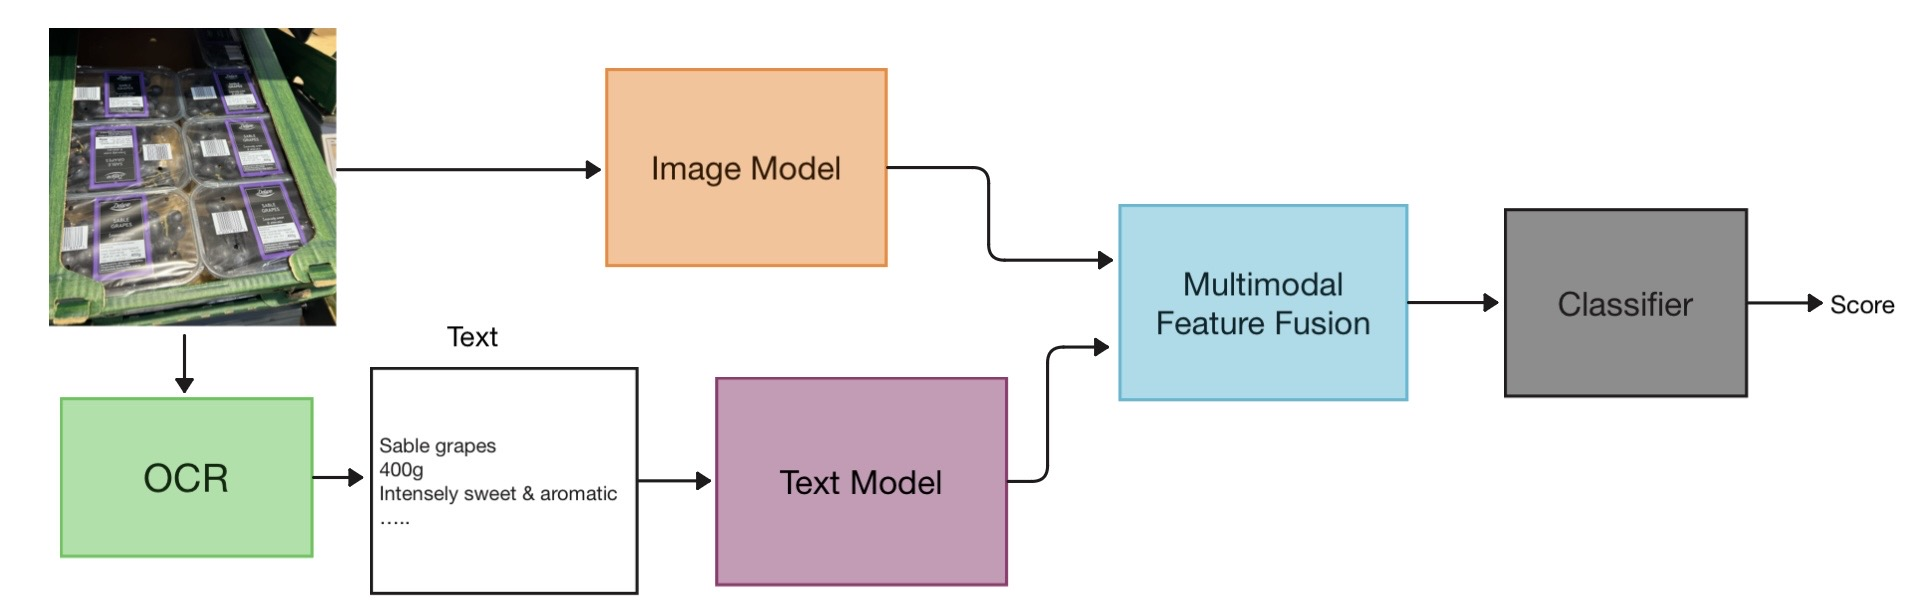
\includegraphics[width=0.85\textwidth]{overall.jpg}
    \caption{Overall multimodal architecture. A product image is processed through two paths: (1) an image model extracts visual features, and (2) OCR extracts text from packaging, which is encoded by a text model. The two feature representations are combined via a multimodal fusion module, and the fused representation is passed to a classifier to produce the product label.}
    \label{fig:overall}
\end{figure*}

% ============================================================================
\section{Background}
\label{sec:background}
% ============================================================================

\subsection{Transfer Learning with CNNs}

When labelled data is limited, training a CNN from scratch leads to overfitting. Transfer learning addresses this by fine-tuning a network pretrained on ImageNet \citep{krizhevsky2012imagenet}. We use MobileNetV3 \citep{howard2019mobilenet}, a lightweight architecture designed for mobile deployment. MobileNetV3 outputs a 1,024-dimensional feature vector after global average pooling, which we project to a 256-dimensional embedding:
\begin{equation}
    \mathbf{x}_{\text{img}} = \text{LN}(\text{Drop}(\text{ReLU}(W_p \cdot \text{Pool}(f(\mathbf{I})))))
\end{equation}
where $f$ is the pretrained backbone and $W_p \in \mathbb{R}^{256 \times 1024}$.

\subsection{Transformer-Based Text Encoding}

We encode OCR text using TinyBERT \citep{jiao2020tinybert}, a distilled BERT model \citep{devlin2019bert} with 4 transformer layers and 312 hidden dimensions. The \texttt{[CLS]} token representation is projected to produce the text embedding:
\begin{equation}
    \mathbf{x}_{\text{txt}} = \text{LN}(\text{Drop}(\text{ReLU}(W_t \cdot \mathbf{h}_{\text{[CLS]}}))) \in \mathbb{R}^{256}
\end{equation}
To regularise on our small dataset, we freeze the first $N$ of TinyBERT's 4 transformer layers, systematically varying $N \in \{0, 1, 2, 3, 4\}$ to find the optimal tradeoff between adaptation and regularisation.

\subsection{Multimodal Fusion}

Fusion methods can be categorised into three types \citep{pettersson2024multimodal}:

\begin{itemize}[nosep,leftmargin=*]
    \item \textbf{Early fusion}: raw features from both modalities are concatenated before any processing.
    \item \textbf{Late fusion}: separate classifiers produce independent predictions that are aggregated (e.g., by averaging or voting).
    \item \textbf{Cross-modal fusion}: intermediate features from both modalities interact during learning, allowing complex cross-modal relationships.
\end{itemize}

Our four fusion strategies span this spectrum: concatenation is an early fusion method, score fusion is a form of late fusion, and gated and cross-attention fusion are cross-modal approaches.

% ============================================================================
\section{Dataset and Task}
\label{sec:dataset}
% ============================================================================

\subsection{Dataset}

We use the GroceryStoreDataset introduced by \citet{klasson2019hierarchical}, a publicly available collection of 5,421 images covering 81 fine-grained product classes organised into a three-level hierarchy: coarse-grained category (e.g., Fruit), fine-grained category (e.g., Apple), and product instance (e.g., Royal Gala). The images were captured in real grocery stores using mobile phone cameras under naturalistic conditions, including varying lighting, viewpoints, and degrees of clutter.

The dataset contains a natural mix of product types: packaged items (milk cartons, juice bottles, yoghurt containers) that typically have visible text on their packaging, and unpackaged items (fruits and vegetables) that have no packaging text. This makes it particularly suitable for studying multimodal fusion, as it requires architectures that can leverage text when available while still performing well without it.

We use the official dataset splits: 2,640 images for training, 2,485 for testing, and an additional 296 validation images provided separately in the dataset (5,421 images in total across all three splits). The number of images per class ranges from 30 to 138, with an average of approximately 32 training images per class.

\subsection{OCR Preprocessing}

We extract text from all images using PaddleOCR and cache the results. Only 37\% of images yield non-empty OCR text. As shown in Figure~\ref{fig:ocr_coverage}, OCR coverage varies dramatically by product category: packaged goods (dairy, juice, yoghurt) achieve 91\% coverage, while fruits (12\%) and vegetables (8\%) rarely yield text. This means that for the majority of images, the multimodal models must rely on visual features alone, making it essential that fusion architectures degrade gracefully when text is absent. The dataset also contains Swedish packaging, which presents an additional challenge for OCR and text matching.

\begin{figure}[t]
    \centering
    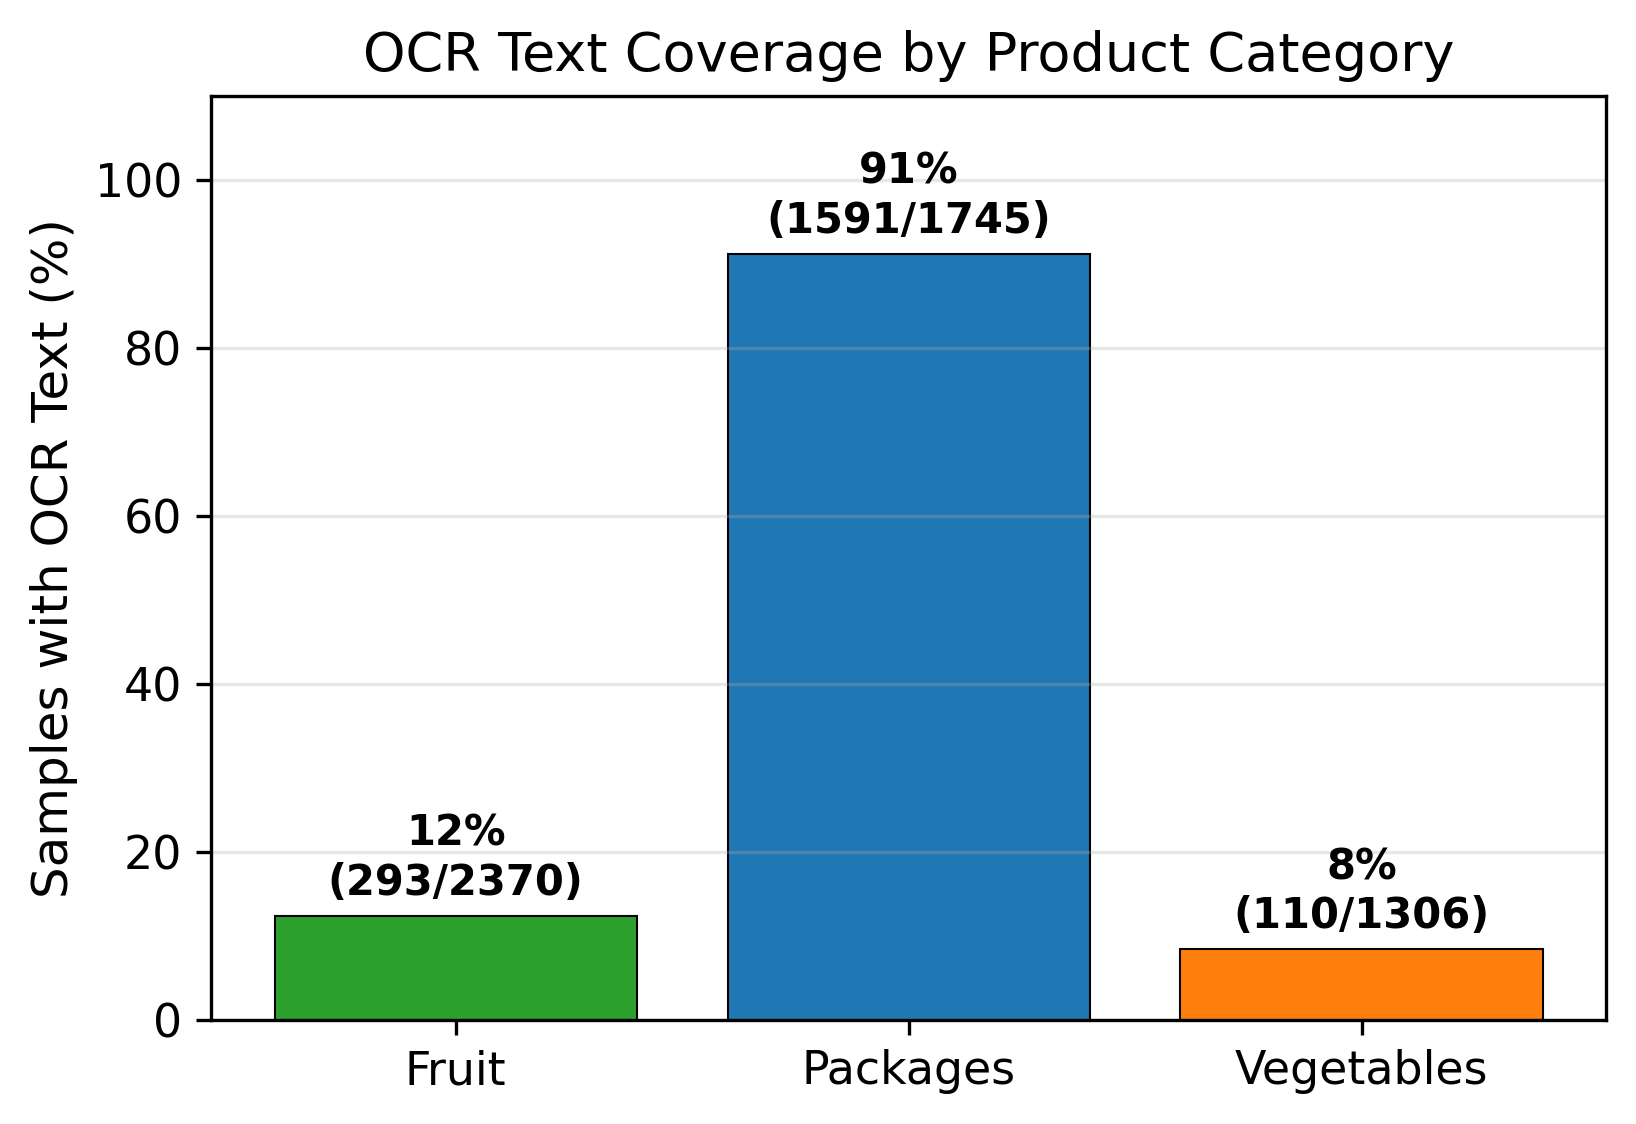
\includegraphics[width=0.85\columnwidth]{ocr_coverage_by_category.png}
    \caption{OCR text coverage by product category. Packaged goods have near-complete coverage (91\%), while unpackaged produce rarely yields text. This asymmetry is the central challenge for multimodal fusion on this dataset.}
    \label{fig:ocr_coverage}
\end{figure}

\subsection{Task and Evaluation Metrics}

Given a single image of a grocery product, the system must classify it into one of 81 fine-grained product classes. We evaluate all models using:
\begin{itemize}[nosep,leftmargin=*]
    \item \textbf{Top-1 accuracy}: percentage of correctly classified test samples.
    \item \textbf{Top-5 accuracy}: percentage of samples where the correct class appears in the top 5 predictions.
    \item \textbf{Macro F1}: unweighted mean of per-class F1 scores, giving equal weight to each class regardless of sample count.
    \item \textbf{Weighted F1}: sample-weighted mean of per-class F1 scores.
\end{itemize}


% ============================================================================
\section{Methodology}
\label{sec:method}
% ============================================================================

\subsection{System Overview}

Our system takes a single product image as input, extracts visual features using a pretrained CNN, and optionally incorporates OCR text to produce a fine-grained classification. The architecture is modular: a shared image encoder and text encoder feed into an interchangeable fusion module, followed by a classification head. We evaluate four fusion strategies while keeping the encoders and classifier fixed, ensuring a fair comparison.

\subsection{Fusion Strategies}

\subsubsection{Concatenation Fusion}

The simplest approach concatenates the image and text embeddings and projects the result:
\begin{equation}
    \mathbf{x}_{\text{fused}} = \text{LN}(\text{Drop}(\text{ReLU}(W_c [\mathbf{x}_{\text{img}}; \mathbf{x}_{\text{txt}}])))
\end{equation}
where $[\cdot;\cdot]$ denotes concatenation and $W_c \in \mathbb{R}^{256 \times 512}$. This imposes no inductive bias about modality importance; the downstream classifier must learn how to weight the features. Its simplicity makes it a useful baseline, but it cannot dynamically adjust when one modality is uninformative (Figure~\ref{fig:concat}).

\begin{figure*}[t]
    \centering
    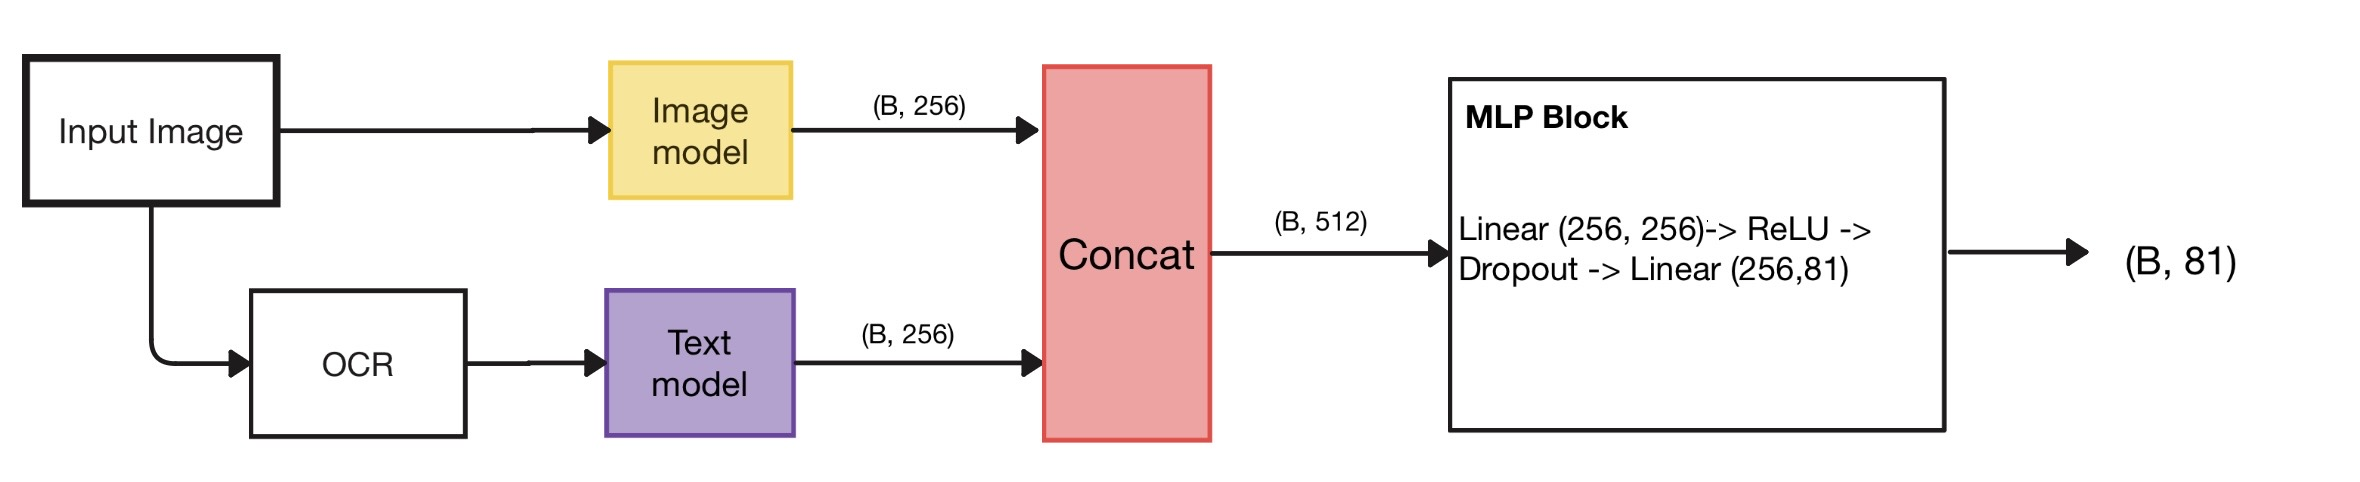
\includegraphics[width=0.75\textwidth]{concat.jpg}
    \caption{Concatenation fusion. Image and text embeddings (each $\mathbb{R}^{256}$) are concatenated to form a 512-dimensional vector, then projected to 256 dimensions by an MLP block for classification.}
    \label{fig:concat}
\end{figure*}

\subsubsection{Gated Fusion}

Gated fusion introduces a learned gate that dynamically weights each modality's contribution. This is motivated by the observation that OCR text is informative for some products (e.g., milk variants distinguished by fat percentage) but absent for others (e.g., unpackaged fruits). Both modalities are first projected to a common space:
\begin{align}
    \mathbf{h}_{\text{img}} &= \text{ReLU}(W_{\text{img}} \mathbf{x}_{\text{img}}) \\
    \mathbf{h}_{\text{txt}} &= \text{ReLU}(W_{\text{txt}} \mathbf{x}_{\text{txt}})
\end{align}
A gating vector is computed from their concatenation:
\begin{equation}
    \mathbf{g} = \sigma(W_g [\mathbf{h}_{\text{img}}; \mathbf{h}_{\text{txt}}]) \in [0, 1]^{256}
\end{equation}
where $\sigma$ is the sigmoid function. The fused representation is the element-wise weighted combination:
\begin{equation}
    \mathbf{x}_{\text{fused}} = \text{LN}(\text{Drop}(\mathbf{g} \odot \mathbf{h}_{\text{img}} + (1 - \mathbf{g}) \odot \mathbf{h}_{\text{txt}}))
\end{equation}

When the text modality is uninformative (e.g., a \texttt{[UNK]} placeholder for unpackaged fruit), the gate can learn values close to 1, effectively reducing the model to image-only classification (Figure~\ref{fig:gated}).

\begin{figure*}[t]
    \centering
    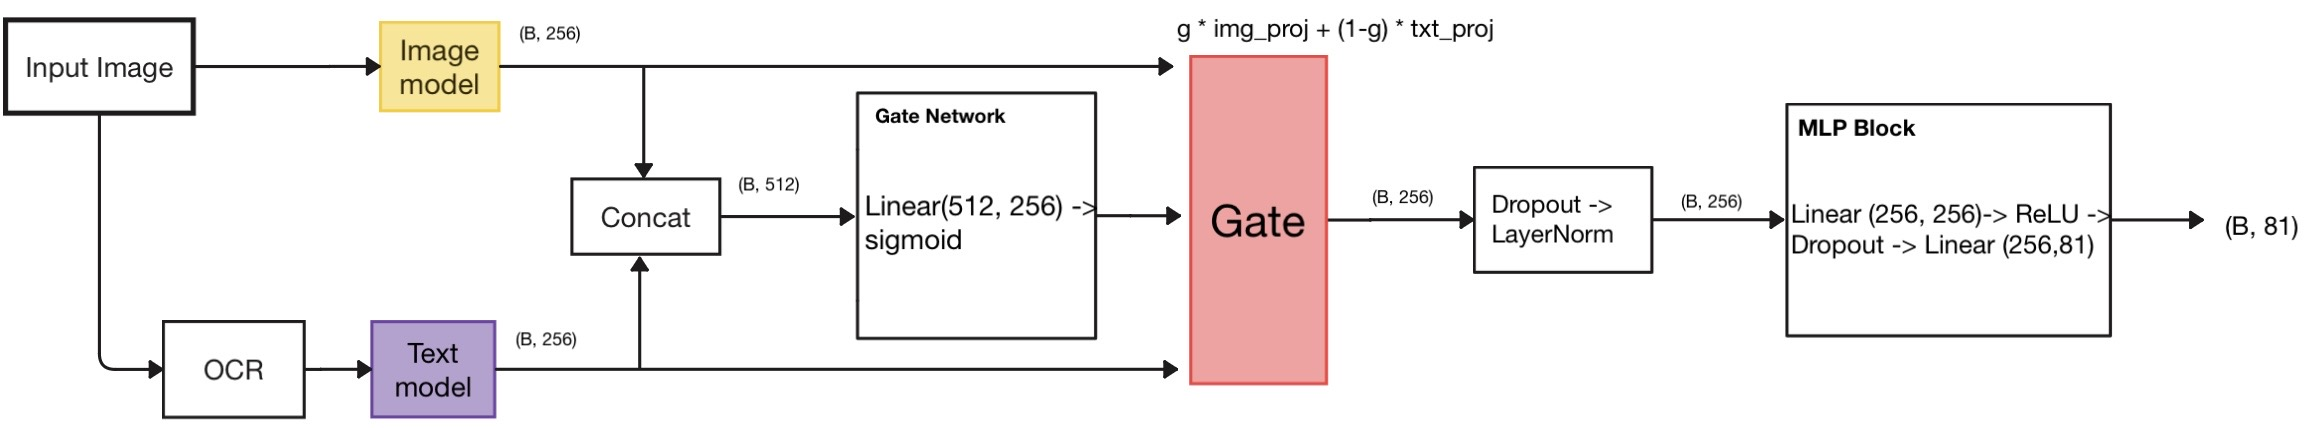
\includegraphics[width=\textwidth]{gated.jpg}
    \caption{Gated fusion. Both modalities are projected to a common space, then a sigmoid gate $\mathbf{g}$ computed from their concatenation dynamically weights the contribution of each modality to the fused representation.}
    \label{fig:gated}
\end{figure*}

\subsubsection{Cross-Attention Fusion}

Cross-attention is the most expressive strategy, operating on token-level sequences from both modalities rather than pooled embeddings. This enables fine-grained interactions---for example, a colour region on packaging might attend to ``strawberry'' in the OCR output.

For cross-attention, both encoders produce sequences instead of single vectors: the image encoder outputs spatial features $\mathbf{X}_{\text{img}} \in \mathbb{R}^{S_{\text{img}} \times 256}$ (reshaped from CNN feature maps), and the text encoder outputs all token embeddings $\mathbf{X}_{\text{txt}} \in \mathbb{R}^{S_{\text{txt}} \times 256}$. Two cross-attention operations are performed using multi-head attention with 4 heads:
\begin{align}
    \tilde{\mathbf{X}}_{\text{img}} &= \text{MHA}(Q\!=\!\mathbf{X}_{\text{img}}, K\!=\!\mathbf{X}_{\text{txt}}, V\!=\!\mathbf{X}_{\text{txt}}) \\
    \tilde{\mathbf{X}}_{\text{txt}} &= \text{MHA}(Q\!=\!\mathbf{X}_{\text{txt}}, K\!=\!\mathbf{X}_{\text{img}}, V\!=\!\mathbf{X}_{\text{img}})
\end{align}
The attended sequences are pooled (mean pooling for image tokens; masked mean pooling for text tokens to handle padding) and combined:
\begin{equation}
    \mathbf{x}_{\text{fused}} = f_{\text{out}}([\text{Pool}(\tilde{\mathbf{X}}_{\text{img}}); \text{MPool}(\tilde{\mathbf{X}}_{\text{txt}})])
\end{equation}
where $f_{\text{out}}$ is a linear projection with ReLU, dropout, and layer normalisation. While cross-attention is the most expressive, it is also the most computationally expensive and potentially data-hungry, which may limit its effectiveness on our small dataset (Figure~\ref{fig:crossattn}).

\begin{figure*}[t]
    \centering
    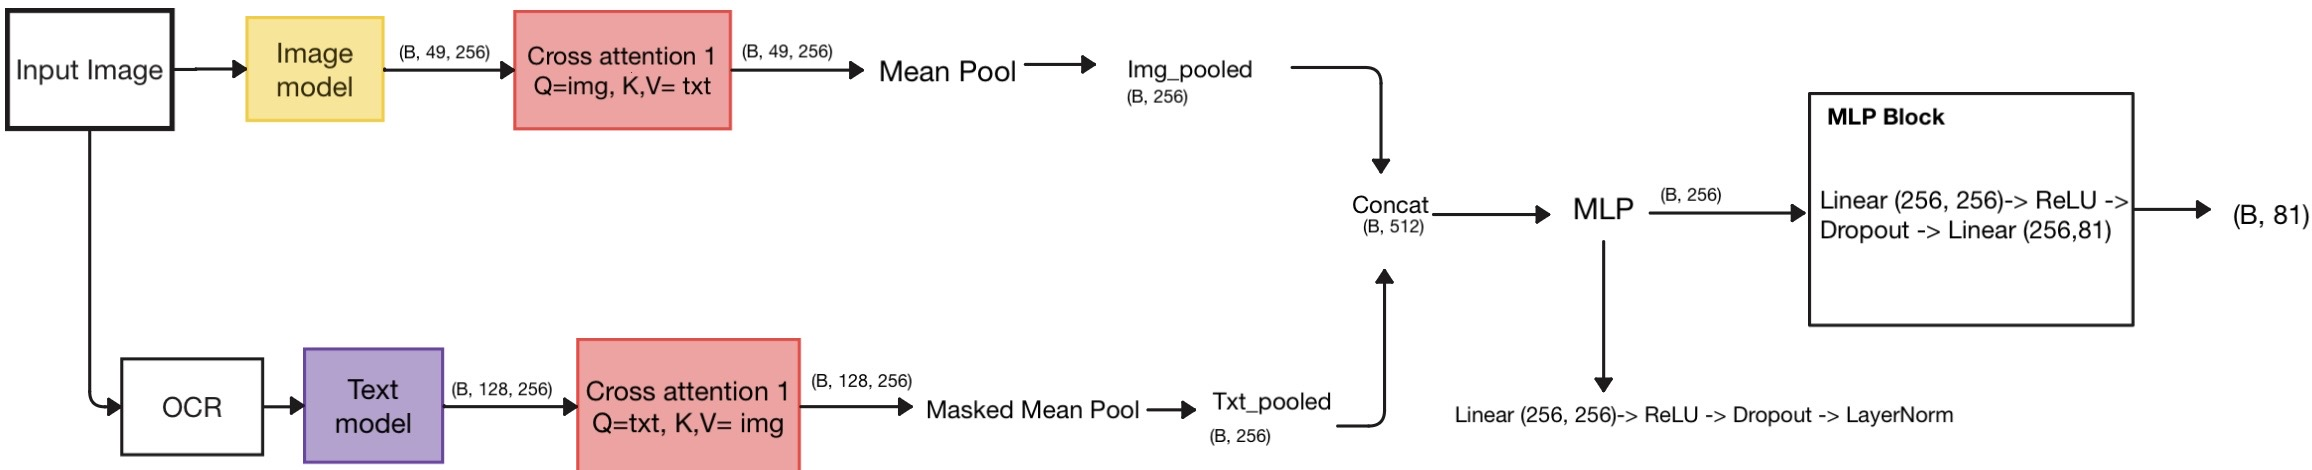
\includegraphics[width=\textwidth]{cross_attention.jpg}
    \caption{Cross-attention fusion. Image spatial features and text token sequences attend to each other via multi-head attention, are mean-pooled, and concatenated before the classification MLP.}
    \label{fig:crossattn}
\end{figure*}

\subsubsection{Score Fusion (Fuzzy Matching)}

Score fusion takes a fundamentally different approach by replacing the learned text encoder with a non-parametric fuzzy string matcher. For each of the 81 product classes, we define a set of known names and aliases $\mathcal{A}_c$ (including Swedish translations, since the GroceryStoreDataset contains Swedish packaging). Given OCR text, the scorer computes a similarity against each class:
\begin{equation}
    s_c = \max_{a \in \mathcal{A}_c} \frac{\text{TokenSetRatio}(\text{ocr},\; a)}{100}
\end{equation}
producing a score vector $\mathbf{s} \in [0, 1]^{81}$. This is combined with image classifier logits via a single \emph{learned} scalar parameter:
\begin{equation}
    \mathbf{y} = \mathbf{y}_{\text{img}} + \alpha \cdot \mathbf{s}
\end{equation}
Crucially, $\alpha$ is \emph{not} a fixed hyperparameter---it is a trainable parameter initialised to 0 and optimised end-to-end via backpropagation alongside the image encoder. This means the model starts as a pure image classifier and the optimiser gradually discovers the appropriate weight for the text signal based on the training data. The final learned value of $\alpha$ serves as interpretable evidence of how much the fuzzy text scores contribute: a large positive $\alpha$ indicates that text matching is a useful complementary signal, while a value near zero would indicate the model found text unreliable. This avoids the need for manual tuning of modality weights. For samples without OCR text, $\mathbf{s}$ is zeroed out, ensuring clean fallback to image-only prediction.

This approach has two practical advantages: (1) no text encoder at inference time, reducing model size and latency; (2) interpretable per-class scores. Its disadvantage is requiring predefined class names, limiting scalability (Figure~\ref{fig:scorefusion}).

\begin{figure*}[t]
    \centering
    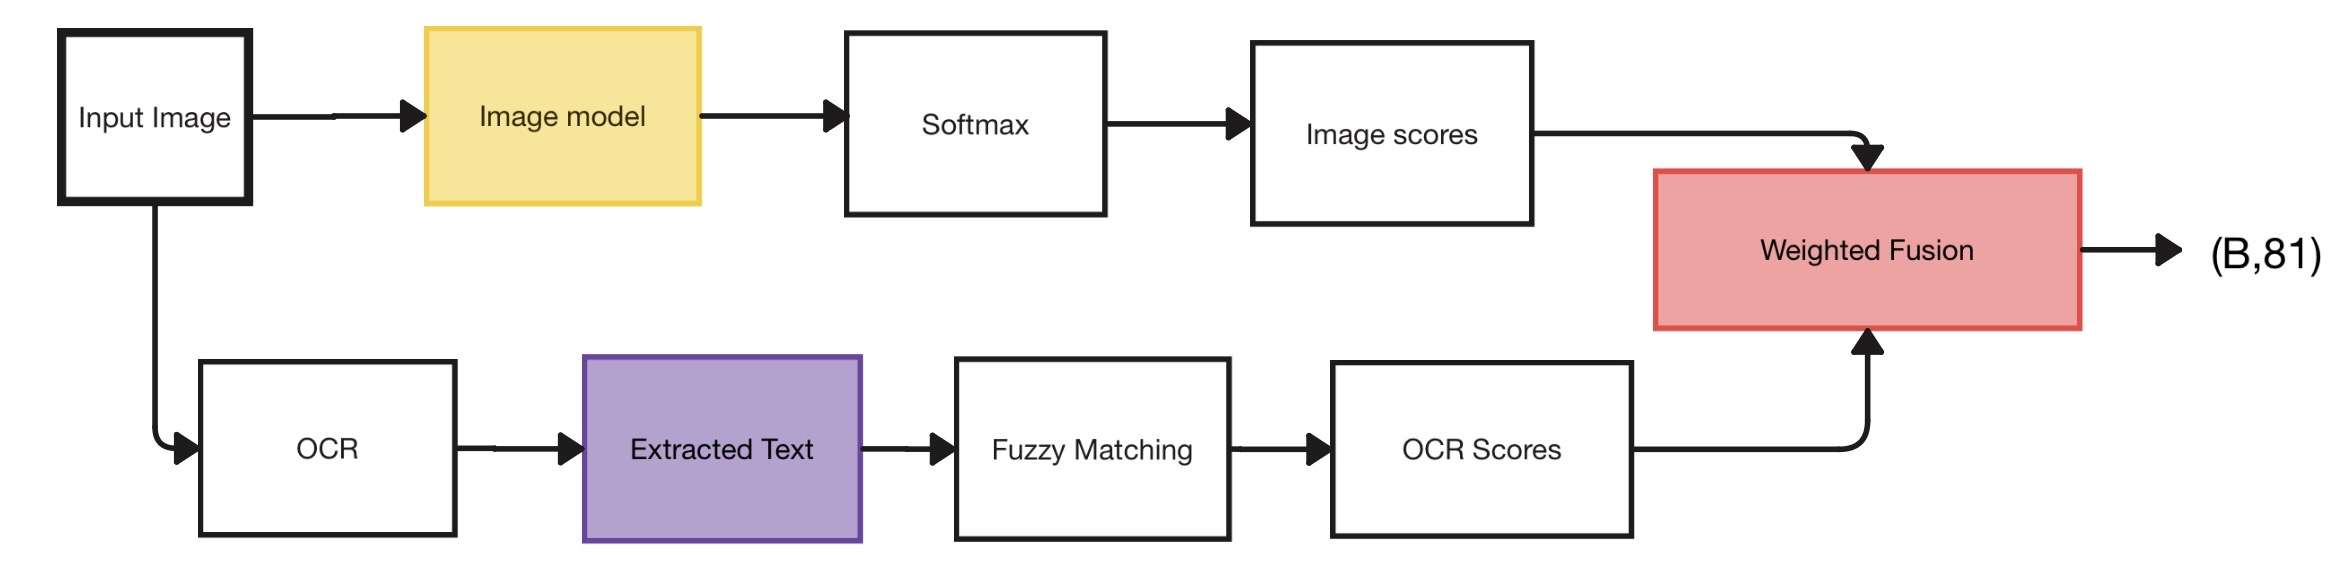
\includegraphics[width=0.85\textwidth]{OCR_score_macthing.jpg}
    \caption{Score fusion. The image path produces class scores via a CNN and softmax, while the text path uses fuzzy string matching against known class names. The two score vectors are combined via a learned weighted fusion ($\alpha$).}
    \label{fig:scorefusion}
\end{figure*}

\subsection{Classification Head}

For all neural fusion strategies, $\mathbf{x}_{\text{fused}} \in \mathbb{R}^{256}$ is passed through a two-layer classifier:
\begin{equation}
    \mathbf{y} = W_2 \cdot \text{Drop}(\text{ReLU}(W_1 \mathbf{x}_{\text{fused}}))
\end{equation}
where $W_1 \in \mathbb{R}^{256 \times 256}$, $W_2 \in \mathbb{R}^{81 \times 256}$, and dropout $p = 0.5$.

\subsection{Training Strategy}

\subsubsection{Addressing Overfitting}

With only ${\sim}32$ images per class, overfitting is the primary challenge. We employ a multi-pronged strategy:

\begin{itemize}[nosep,leftmargin=*]
    \item \textbf{Staged pretraining} of encoders before end-to-end training.
    \item \textbf{Data augmentation}: 8 strategies (Table~\ref{tab:augmentation}).
    \item \textbf{Heavy regularisation}: dropout ($p = 0.3$--$0.5$), label smoothing ($\epsilon = 0.1$), weight decay ($10^{-4}$), gradient clipping.
    \item \textbf{Text encoder layer freezing} to preserve pretrained representations.
    \item \textbf{Compact models}: TinyBERT (14.5M params), MobileNetV3 (2.5M params).
    \item \textbf{Early stopping} with patience of 15 epochs.
    \item \textbf{Differential learning rates}: $0.1\times$ for pretrained encoders.
\end{itemize}

\noindent As shown in Table~\ref{tab:overfitting}, all models exhibit train-val gaps in the 14--16\% range, indicating controlled overfitting.

\begin{table}[t]
\centering
\caption{Train-val accuracy gap at best epoch. All gaps are in a narrow 14--16\% range, indicating controlled overfitting.}
\label{tab:overfitting}
\small
\begin{tabular}{@{}lcccc@{}}
\toprule
\textbf{Model} & \textbf{Epoch} & \textbf{Train} & \textbf{Val} & \textbf{Gap} \\
\midrule
Image-only   & 44 & 84.06 & 70.65 & 14.41 \\
Concat       & 43 & 88.82 & 73.30 & 15.52 \\
Gated        & 29 & 88.62 & 73.01 & 15.01 \\
Cross-attn   & 42 & 89.33 & 74.65 & 14.68 \\
Score fusion & 36 & 92.40 & 77.64 & 14.76 \\
\bottomrule
\end{tabular}
\end{table}

\subsubsection{Staged Training}

In Stage~1, encoders are pretrained independently for 20 epochs (text encoder on OCR-text samples only). An auxiliary spatial head ensures the image encoder's spatial projection receives gradients for cross-attention. In Stage~2, the full model trains end-to-end with differential learning rates ($1 \times 10^{-5}$ for encoders, $1 \times 10^{-4}$ for fusion/classifier).

\subsubsection{Data Augmentation}

Table~\ref{tab:augmentation} lists the augmentation pipeline, which simulates realistic capture conditions. Mixup \citep{zhang2018mixup} is applied to 50\% of batches but disabled for cross-attention (mixed images do not correspond to text tokens).

\begin{table}[t]
\centering
\caption{Data augmentation pipeline applied during training.}
\label{tab:augmentation}
\small
\begin{tabular}{@{}ll@{}}
\toprule
\textbf{Augmentation} & \textbf{Parameters} \\
\midrule
RandomResizedCrop & scale $[0.7, 1.0]$ \\
RandomHorizontalFlip & $p = 0.5$ \\
RandomRotation & $\pm 15^{\circ}$ \\
RandomPerspective & distortion $0.2$, $p = 0.3$ \\
ColorJitter & bright. $0.3$, contr. $0.3$ \\
GaussianBlur & $\sigma \in [0.1, 2.0]$ \\
Cutout & 1 hole, $32 \!\times\! 32$ px \\
Mixup & $\alpha = 0.2$, 50\% of batches \\
\bottomrule
\end{tabular}
\end{table}

The learning rate follows a linear warmup over 5 epochs followed by cosine annealing.


% ============================================================================
\section{Experiments}
\label{sec:experiments}
% ============================================================================

All experiments use the hyperparameters summarised in Table~\ref{tab:hyperparams}. To reduce the number of experimental variables and focus on the impact of fusion strategy, we keep the image backbone (MobileNetV3), text model (TinyBERT), embedding dimensions (256), and training procedure fixed across all experiments. All experiments are conducted on an NVIDIA GeForce RTX 3060 Laptop GPU (6\,GB VRAM) using a single seed (42), applied to Python, NumPy, and PyTorch CPU/CUDA with \texttt{cudnn.deterministic = True} for reproducibility.

\begin{table}[t]
\centering
\caption{Experimental hyperparameters, fixed across all fusion strategies.}
\label{tab:hyperparams}
\small
\begin{tabular}{@{}ll@{}}
\toprule
\textbf{Parameter} & \textbf{Value} \\
\midrule
Image backbone & MobileNetV3 \\
Text model & TinyBERT (4L, 312D) \\
Embedding dim & 256 \\
Image size & $224 \times 224$ \\
Batch size & 32 \\
Optimiser & AdamW ($\lambda = 10^{-4}$) \\
Stage 1 LR & $3 \times 10^{-4}$ \\
Stage 2 LR (encoders) & $1 \times 10^{-5}$ \\
Stage 2 LR (fusion/cls) & $1 \times 10^{-4}$ \\
Schedule & Warmup (5 ep) + cosine \\
Stage 1 / 2 epochs & 20 / 50 \\
Label smoothing & 0.1 \\
Cross-attn heads & 4 \\
\bottomrule
\end{tabular}
\end{table}

\subsection{Results Overview}

We first compare all five architectures to determine which fusion strategy is most effective for fine-grained grocery classification. Table~\ref{tab:params} summarises the parameter counts and Table~\ref{tab:main_results} reports test set performance.

\begin{table}[t]
\centering
\caption{Parameter counts. Neural fusion models include TinyBERT (${\sim}$12M frozen params). Score fusion adds only 1 parameter ($\alpha$) over the image-only baseline.}
\label{tab:params}
\small
\begin{tabular}{@{}lrr@{}}
\toprule
\textbf{Model} & \textbf{Total} & \textbf{Trainable} \\
\midrule
Image-only      & 2,015,601  & 2,015,601 \\
Concat          & 16,578,329 & 4,610,105 \\
Gated           & 16,709,913 & 4,741,689 \\
Cross-attn      & 17,236,249 & 5,268,025 \\
Score fusion    & 2,015,602  & 2,015,602 \\
\bottomrule
\end{tabular}
\end{table}

\begin{table}[t]
\centering
\caption{Test set performance across all models. Best result in each column is \textbf{bolded}.}
\label{tab:main_results}
\vspace{0.5em}
\small
\begin{tabular}{@{}lcccc@{}}
\toprule
\textbf{Model} & \textbf{Top-1} & \textbf{Top-5} & \textbf{Mac F1} & \textbf{Wt F1} \\
\midrule
Image-only      & 70.12 & 94.33 & 0.6982 & 0.6919 \\
Concat          & 72.77 & 95.12 & 0.7252 & 0.7255 \\
Gated           & 71.45 & 95.07 & 0.7198 & 0.7213 \\
Cross-attn      & 73.54 & 94.68 & 0.7422 & 0.7341 \\
Score fusion    & \textbf{75.61} & \textbf{96.01} & \textbf{0.7692} & \textbf{0.7585} \\
\bottomrule
\end{tabular}
\end{table}

Several patterns emerge. All multimodal methods outperform the image-only baseline, confirming that OCR text provides useful signal. The ranking is: score fusion (75.61\%) $>$ cross-attention (73.54\%) $>$ concatenation (72.77\%) $>$ gated (71.45\%) $>$ image-only (70.12\%). Most strikingly, the simplest text representation (fuzzy string matching) outperforms all three neural approaches, suggesting that on this small dataset, domain knowledge encoded as class-name aliases is more effective than learning text representations from limited, noisy data.

Gated fusion underperforms concatenation despite its additional gating mechanism. Analysis of the learned gate values reveals the cause: the gate converges to a near-static ratio (mean $\approx 0.61$, favouring image) with negligible difference between text-present (0.614) and text-absent (0.608) samples, effectively reducing it to a fixed-weight concatenation. For score fusion, the learned scale $\alpha$ grows monotonically from 0 to 0.264 during training (Figure~\ref{fig:alpha_curve}), confirming that the model discovers the fuzzy text signal to be genuinely useful.

\begin{figure}[t]
    \centering
    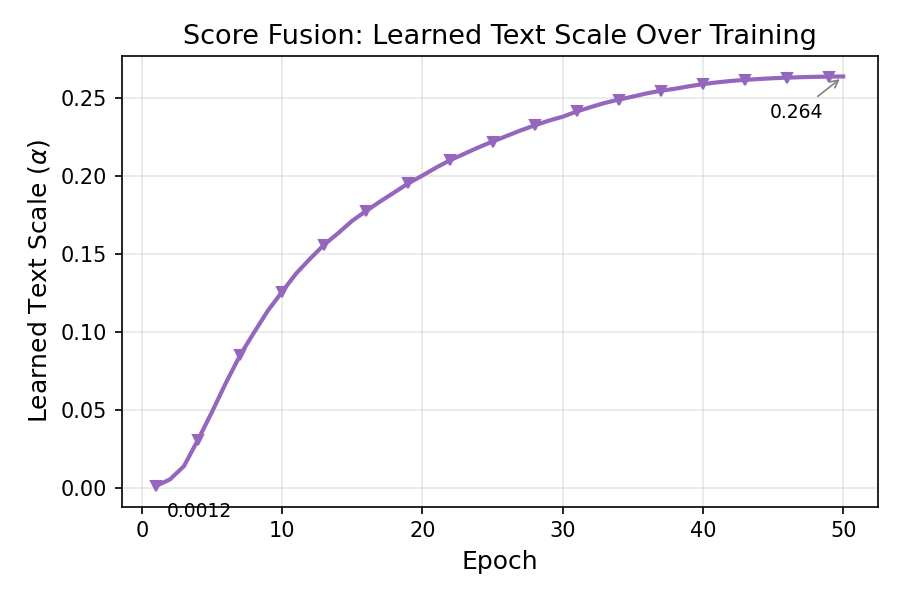
\includegraphics[width=0.85\columnwidth]{score_fusion_alpha.png}
    \caption{Learned text scale $\alpha$ during score fusion training, growing from 0 (pure image classifier) to 0.264. The plateau after epoch 30 indicates convergence.}
    \label{fig:alpha_curve}
\end{figure}

Figures~\ref{fig:training_curves} and~\ref{fig:training_curves_top5} show the validation accuracy curves. All models converge within 50 epochs, with score fusion achieving the highest accuracy early and maintaining its lead. The top-5 curves (Figure~\ref{fig:training_curves_top5}) are tightly grouped above 90\%.

\begin{figure}[t]
    \centering
    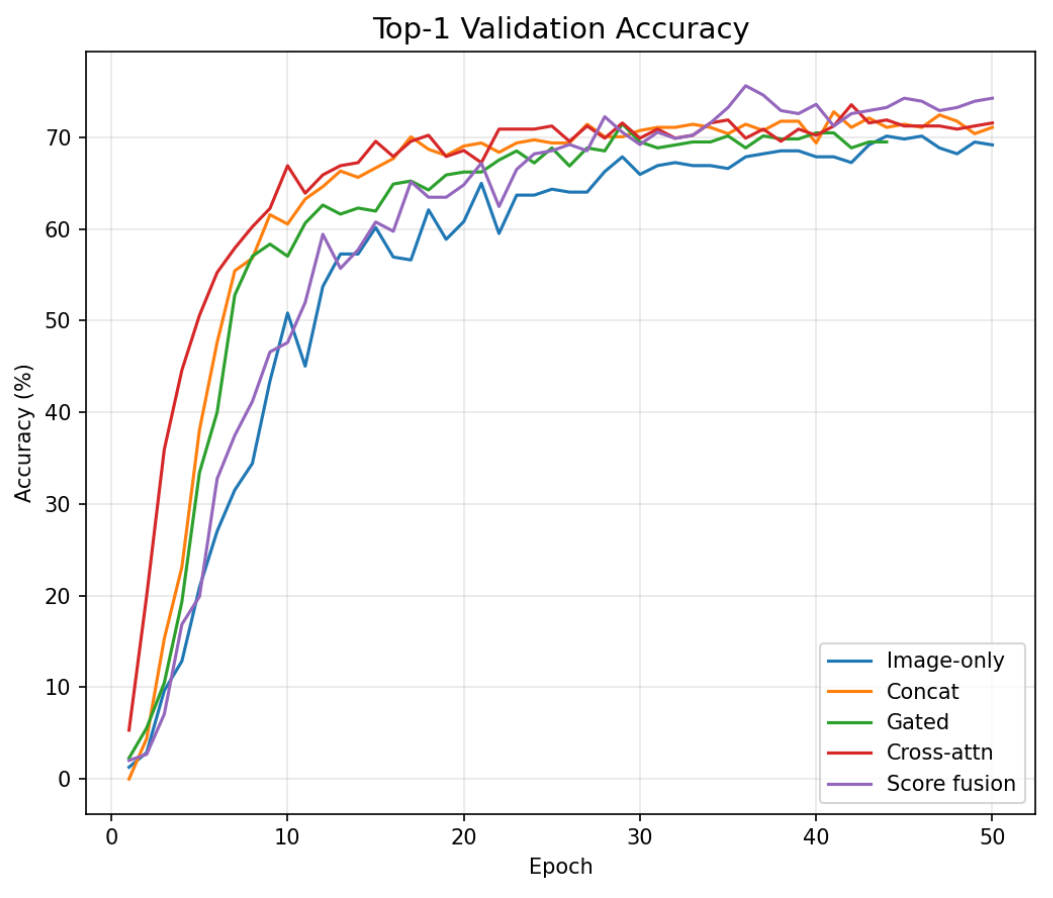
\includegraphics[width=\columnwidth]{training_curve_top1.png}
    \caption{Top-1 validation accuracy during Stage~2 training. Score fusion achieves the highest accuracy and converges smoothly, while the neural fusion methods show more fluctuation.}
    \label{fig:training_curves}
\end{figure}

\begin{figure}[t]
    \centering
    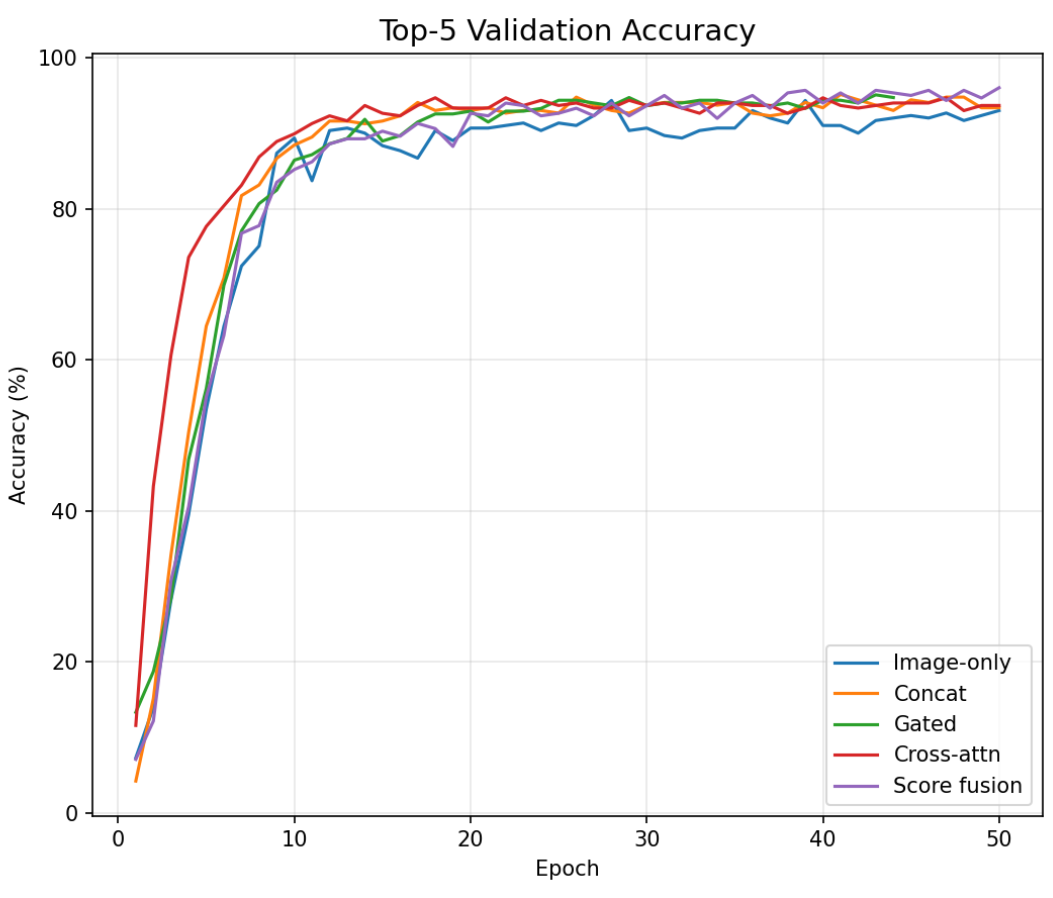
\includegraphics[width=\columnwidth]{training_curve_top5.png}
    \caption{Top-5 validation accuracy during Stage~2 training. All models are tightly grouped above 90\%, confirming that the correct class is reliably among the top predictions.}
    \label{fig:training_curves_top5}
\end{figure}

\subsection{Modality Contribution Analysis}

To isolate when and how much text contributes, we evaluate all models on the subset of test images with non-empty OCR output (Table~\ref{tab:text_subset}), since only 37\% of images have OCR text. This isolates the effect of text fusion on products where text is actually available.

\begin{table}[t]
\centering
\caption{Performance on the text-available subset only (37\% of test images). $\Delta$ is the top-1 improvement over image-only on this subset.}
\label{tab:text_subset}
\small
\begin{tabular}{@{}lcccc@{}}
\toprule
\textbf{Model} & \textbf{Top-1} & \textbf{Top-5} & \textbf{Wt F1} & \textbf{$\Delta$} \\
\midrule
Image-only      & 71.13 & 93.27 & 0.6920 & --- \\
Concat          & 74.29 & 97.90 & 0.7513 & +3.16 \\
Gated           & 74.41 & 96.91 & 0.7497 & +3.28 \\
Cross-attn      & 77.12 & 98.02 & 0.7678 & +5.99 \\
Score fusion    & \textbf{78.90} & 97.69 & \textbf{0.7890} & \textbf{+7.77} \\
\bottomrule
\end{tabular}
\end{table}

Comparing Table~\ref{tab:text_subset} with the full-dataset results in Table~\ref{tab:main_results} reveals how much each fusion strategy benefits from available text. The image-only baseline performs similarly on both subsets (71.13\% vs 70.12\%), confirming that the text-available subset is not inherently easier to classify visually. However, all multimodal methods show larger gains on this subset. Cross-attention improves from +3.42 points over the baseline (full dataset) to +5.99 points (text-available subset)---nearly doubling its advantage. Score fusion shows the largest text-conditional gain at +7.77 points.

This has an important implication: the overall results in Table~\ref{tab:main_results} \emph{underestimate} the value of text fusion, because 63\% of test images have no text and therefore cannot benefit from the text modality. Figure~\ref{fig:per_category} breaks this down by product category. On packaged goods (91\% OCR coverage), all fusion methods substantially outperform image-only, with score fusion achieving 88.3\% (+14.4 points). On fruit and vegetables (8--12\% OCR coverage), the gains are minimal ($<$1 point), confirming that text fusion only helps when text is available. The practical benefit of these models in a BVI assistive application would depend on the proportion of text-bearing products in the user's typical shopping basket.

\begin{figure}[t]
    \centering
    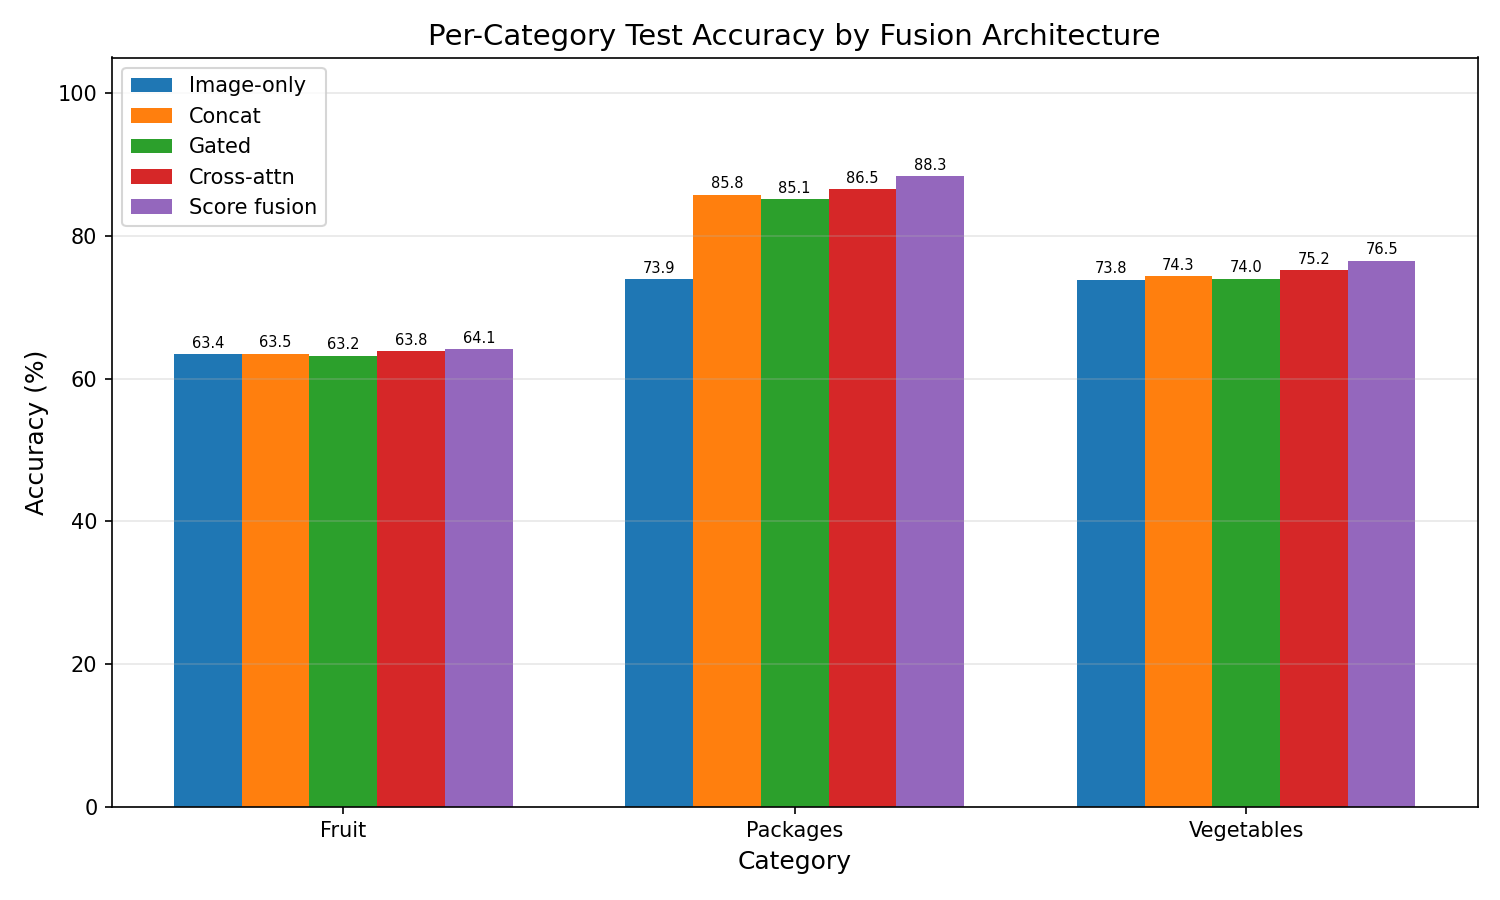
\includegraphics[width=\columnwidth]{per_category_accuracy.png}
    \caption{Per-category test accuracy by fusion architecture. Text fusion provides large gains on packaged goods (which have OCR text) but negligible gains on fruit and vegetables (which do not). This directly mirrors the OCR coverage pattern in Figure~\ref{fig:ocr_coverage}.}
    \label{fig:per_category}
\end{figure}

To further quantify each modality's contribution, we evaluate the three neural fusion models with one modality zeroed out (Table~\ref{tab:modality}). In the ``Image-only'' condition, text embeddings are set to zero; in ``Text-only'', image embeddings are set to zero.

\begin{table}[t]
\centering
\caption{Modality ablation (top-1 accuracy \%). Text $\Delta$ is the gain from adding text to the image-only condition.}
\label{tab:modality}
\small
\begin{tabular}{@{}lcccc@{}}
\toprule
\textbf{Fusion} & \textbf{Full} & \textbf{Img-only} & \textbf{Txt-only} & \textbf{$\Delta$} \\
\midrule
Concat      & 72.77 & 68.52 & 31.24 & +4.25 \\
Gated       & 71.45 & 69.11 & 28.19 & +2.34 \\
Cross-attn  & 73.54 & 67.28 & 27.81 & +6.26 \\
\bottomrule
\end{tabular}
\end{table}

Three findings stand out. First, all fusion methods genuinely use both modalities: the full model consistently outperforms the image-only condition, confirming that none of the architectures have learned to ignore text. Second, cross-attention shows the largest text contribution (+6.26 points) and also the highest text-only accuracy (27.81\%), indicating that its bidirectional attention mechanism produces the richest text representations. However, this reliance on cross-modal interaction comes at a cost: when text is zeroed out, cross-attention drops to the lowest image-only accuracy (67.28\%), below both concatenation (68.52\%) and gated (69.11\%). Third, gated fusion shows the smallest text contribution (+2.34 points) and the highest image-only accuracy (69.11\%), confirming that the gate has learned to rely primarily on image features---making it the most robust to missing or unreliable text, but limiting its ability to exploit text when it is available.

\subsection{Layer Freezing}

To determine how much the text encoder should adapt to noisy OCR input versus preserving its pretrained representations, we systematically vary the number of unfrozen TinyBERT layers. Table~\ref{tab:freezing} shows the effect on weighted F1 across all three neural fusion strategies. TinyBERT has 4 transformer layers; ``0 unfrozen'' means all layers are frozen (text encoder used as a fixed feature extractor), while ``2 unfrozen'' means the top 2 layers are fine-tuned on the OCR data.

\begin{table}[t]
\centering
\caption{Effect of text encoder layer unfreezing on weighted F1. TinyBERT has 4 layers; unfreezing allows adaptation to noisy OCR input. Image-only baseline (0.6919) is independent of text encoder configuration.}
\label{tab:freezing}
\small
\begin{tabular}{@{}lccc@{}}
\toprule
\textbf{Model} & \textbf{0 unfrozen} & \textbf{1 unfrozen} & \textbf{2 unfrozen} \\
\midrule
Image-only      & 0.6919 & 0.6919 & 0.6919 \\
Concat          & 0.7255 & 0.7321 & \textbf{0.7367} \\
Gated           & 0.7213 & 0.7349 & \textbf{0.7416} \\
Cross-attn      & \textbf{0.7341} & 0.7279 & 0.7158 \\
\bottomrule
\end{tabular}
\end{table}

A clear and surprising pattern emerges: concatenation and gated fusion \emph{improve} as more text encoder layers are unfrozen, while cross-attention \emph{degrades}. For concatenation, unfreezing 2 layers improves weighted F1 from 0.7255 to 0.7367 (+1.1 points). Gated fusion shows an even larger gain, from 0.7213 to 0.7416 (+2.0 points)---making it competitive with cross-attention when given the freedom to adapt its text representations. Notably, gated fusion with 2 unfrozen layers (0.7416) surpasses cross-attention at any freezing configuration (best: 0.7341).

Cross-attention tells the opposite story: unfreezing text layers causes weighted F1 to drop from 0.7341 to 0.7158 ($-$1.8 points). This is consistent with overfitting: cross-attention already has the most parameters due to its multi-head attention layers, and unfreezing the text encoder adds further trainable parameters that the small dataset cannot support. For cross-attention, the pretrained frozen text representations provide a more stable signal.

This finding has practical implications: the optimal text encoder configuration depends on the fusion strategy. Simpler fusion methods (concatenation, gated) benefit from text encoder adaptation, while more complex methods (cross-attention) require the regularisation provided by frozen pretrained weights.

% ============================================================================
\section{Qualitative Analysis}
\label{sec:qualitative}
% ============================================================================

Figure~\ref{fig:qualitative} illustrates a case where OCR text corrects an image-only misclassification. The test image shows bags of Granny Smith apples on a shelf, with ``GRANNY SMITH APPLES'' clearly printed on the packaging. The image-only model predicts Anjou pear with 65.8\% confidence---a reasonable visual confusion, since both are green, round fruits. However, all four fusion models correctly identify the product by leveraging the OCR text. Score fusion achieves the highest confidence (92.8\%), demonstrating the core value of multimodal fusion: packaging text provides a discriminative signal that the image alone cannot.

\begin{figure}[t]
    \centering
    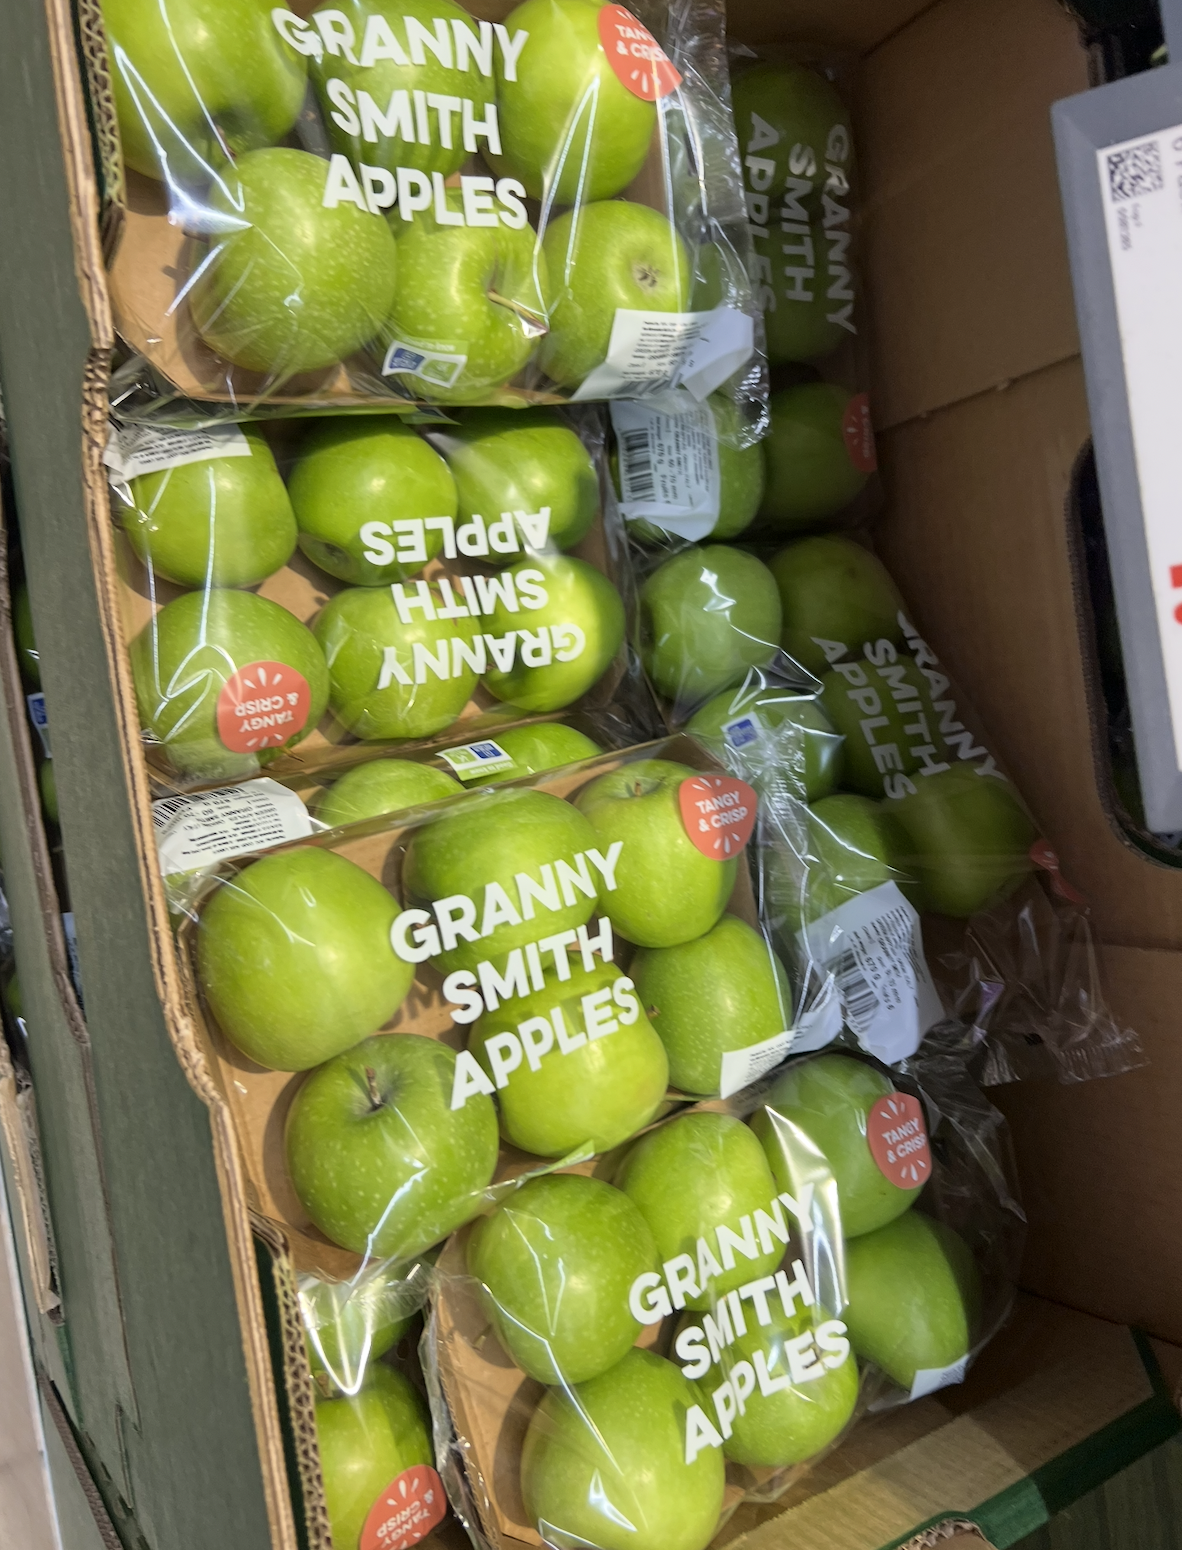
\includegraphics[width=0.85\columnwidth, trim=0 250 0 250, clip]{granny_smith_apples.png}

    \vspace{0.5em}
    \small
    \begin{tabular}{@{}lcc@{}}
    \toprule
    \textbf{Model} & \textbf{Top-1 Prediction} & \textbf{Confidence} \\
    \midrule
    Image-only      & Anjou (pear)          & 65.8\% \\
    Concat          & Granny-Smith          & 87.4\% \\
    Gated           & Granny-Smith          & 85.8\% \\
    Cross-attn      & Granny-Smith          & 84.6\% \\
    Score fusion    & Granny-Smith          & 92.8\% \\
    \bottomrule
    \end{tabular}

    \caption{Qualitative example. \textit{Top:} bags of Granny Smith apples with clear text on packaging. \textit{Bottom:} model predictions. OCR extracted ``GRANNY SMITH APPLES''. The image-only baseline misclassifies this as Anjou (a green pear), while all four fusion models correctly identify Granny Smith.}
    \label{fig:qualitative}
\end{figure}

% ============================================================================
\section{Related Work}
\label{sec:related_work}
% ============================================================================

\citet{klasson2019hierarchical} introduced the GroceryStoreDataset and benchmarked CNN classifiers; \citet{klasson2020using} later improved accuracy by combining images with web-scraped text descriptions, though this assumes pre-collected descriptions. \citet{georgiadis2021products6k} benchmarked OCR-based re-ranking on Products-6K, and \citet{george2015fine} pioneered OCR for grocery recognition using word frequency histograms.

Most relevant to our work, \citet{pettersson2024multimodal} compared concatenation and gated fusion across multiple image and text models on their FineGrainOCR dataset, finding that multimodal approaches outperform unimodal baselines. We follow a similar methodology but differ in four respects: (1) we use the publicly available GroceryStoreDataset; (2) we include cross-attention fusion, which they did not evaluate; (3) we include a non-parametric score fusion approach; and (4) we investigate layer freezing as regularisation. A persistent challenge across all OCR-based methods is text quality on grocery products (curved surfaces, small fonts, multilingual text) and the absence of packaging text on fruits and vegetables.

% ============================================================================
\section{Discussion \& Conclusions}
\label{sec:conclusion}
% ============================================================================

\subsection{Summary}

Returning to our research question---\emph{which fusion strategy best combines visual and OCR features, and under what conditions does each succeed or fail?}---we compared four multimodal fusion strategies for fine-grained grocery product identification. Score fusion achieves the best accuracy (75.61\%), outperforming the image-only baseline by +5.5 points and cross-attention (the best neural method) by +2.1 points. Score fusion's success stems from three factors: (1) fuzzy matching exploits prior knowledge of class names rather than learning from limited, noisy OCR data; (2) curated Swedish aliases encode domain knowledge; and (3) its single-parameter architecture is highly resistant to overfitting. The layer freezing analysis reveals fusion-dependent optimal configurations: simpler methods benefit from unfreezing text layers, while cross-attention degrades due to overfitting.

\subsection{When Does Text Help?}

Text fusion primarily helps packaged products (Figure~\ref{fig:per_category}): on the 37\% of images with OCR text, score fusion improves by +7.77 points over image-only, versus +5.49 on the full dataset. Cross-attention benefits most from text (+6.26 points, Table~\ref{tab:modality}) but is most damaged when text is removed. Gated fusion benefits least (+2.34 points) but is most robust to missing text. The 63\% of images without text (fruits and vegetables) dilute the overall multimodal advantage.

\subsection{Limitations and Future Work}

Our evaluation is limited to a single dataset (${\sim}5,400$ images, 81 classes), a single OCR engine, and a single random seed. The fuzzy scorer requires manually curated class-name aliases, limiting scalability. Compared to \citet{pettersson2024multimodal}, whose larger dataset favours neural fusion, our results suggest the optimal strategy is dataset-size-dependent. Future work should evaluate on larger datasets, investigate end-to-end OCR training, and conduct user studies with BVI participants.


% ============================================================================
\bibliography{refs}

% ============================================================================

\end{document}
